\documentclass[11pt,a4paper]{article}
\usepackage[T1]{fontenc}
\usepackage{lmodern,microtype}
\usepackage[margin=24mm,headheight=14pt]{geometry}
\usepackage{amsmath,amssymb,booktabs,array,tabularx}
\usepackage{xcolor,tikz,fancyhdr,enumitem}
\usepackage[colorlinks=true,linkcolor=teal,urlcolor=teal]{hyperref}
\usetikzlibrary{arrows.meta,positioning}
\definecolor{ink}{HTML}{15354A}
\definecolor{teal}{HTML}{007E87}
\definecolor{pale}{HTML}{EDF5F6}
\hypersetup{pdftitle={FluidDynamicsMetal: Equations and Real-Time Approximations},
 pdfauthor={FluidDynamicsMetal project},pdfsubject={A source-based explanation of the Metal fluid simulation}}
\pagestyle{fancy}\fancyhf{}
\fancyhead[L]{\small\sffamily\color{ink}FluidDynamicsMetal}
\fancyhead[R]{\small\sffamily Equations and approximations}
\fancyfoot[L]{\footnotesize Source-based technical note\quad\textbar\quad 26 September 2026}
\fancyfoot[R]{\small\thepage}
\renewcommand{\headrulewidth}{0.3pt}
\setlength{\parindent}{0pt}
\setlength{\parskip}{6pt}
\setlist[itemize]{leftmargin=1.3em,itemsep=3pt,topsep=3pt}
\setlist[enumerate]{leftmargin=1.5em,itemsep=3pt,topsep=3pt}
\newcommand{\uvec}{\mathbf{u}}
\newcommand{\xvec}{\mathbf{x}}
\newcommand{\src}[1]{\par{\footnotesize\raggedright\color{teal}\textbf{Source:} #1\par}}
\newcommand{\code}[1]{\texttt{#1}}
\newcommand{\note}[1]{\par\smallskip\noindent\colorbox{pale}{\parbox{\dimexpr\linewidth-2\fboxsep\relax}{#1}}\par\smallskip}
\newcommand{\page}[1]{\clearpage\section{#1}}
\newcolumntype{Y}{>{\raggedright\arraybackslash}X}
\begin{document}
\thispagestyle{empty}
{\sffamily\color{teal}\large IMPLEMENTATION GUIDE}\par
\vspace{7mm}
{\sffamily\bfseries\color{ink}\Huge FluidDynamicsMetal}\par
\vspace{3mm}
{\sffamily\color{ink}\LARGE Equations and real-time approximations}\par
\vspace{5mm}
{\large How the Swift renderer and Metal shaders create moving dye}\par
\vspace{5mm}
\textbf{Source snapshot:} \code{9477dabc41a2} \quad\textbar\quad 26 September 2026

\section*{What this simulation represents}
The app evolves a two-dimensional velocity field and a scalar dye field on a
rectangular grid. Pointer or touch motion adds local velocity; contact also adds
dye. Advection carries both fields, an artificial swirl force restores visible
rotation, and a pressure-like correction reduces compression and expansion.
The final image is a colour mapping of one stored field.

This is a visual fluid model inspired by incompressible flow. It does not model a
water surface, three-dimensional smoke, variable mass density, or calibrated
physical units. In particular, the field called \emph{Density} is transported dye,
not the fluid's mass density.

\note{\textbf{Reading rule.} The source code is the authority throughout this
document. Continuum equations explain the intended model; discrete equations
describe the actual shader operations. Consequences inferred from those
operations are identified as numerical limitations, not as measured errors.}

\section*{Reading map}
\begin{tabularx}{\linewidth}{@{}rY@{}}
\toprule
Page & Topic \\
\midrule
2 & The underlying fluid and dye equations \\
3 & Grid coordinates, stored fields, and the exact frame sequence \\
4 & Backward advection and bilinear interpolation \\
5 & Contact forces, dye injection, and fading \\
6 & Vorticity confinement and boundaries \\
7 & Pressure projection and the 40-step Jacobi solve \\
8 & Why incompressibility and conservation are approximate \\
9 & GPU execution, precision, initial state, and resizing \\
10 & Displayed fields and the actual tuning parameters \\
11 & Source map, scope of verification, and rebuilding this PDF \\
\bottomrule
\end{tabularx}

\vfill
{\small The shared simulation sources compile into both the Mac and iOS apps.
Platform input handling differs, but the numerical shaders and frame pipeline
described here are shared. This document is self-contained; external reading is
optional.}

\page{From fluid mechanics to a visual model}
Let $\uvec=(u,v)$ be velocity, $p$ physical pressure, $\rho_0$ constant fluid mass
density, $\nu$ kinematic viscosity, and $\mathbf f$ force per unit mass. The
incompressible Navier--Stokes model in two dimensions is
\begin{align}
 \frac{\partial\uvec}{\partial t}+(\uvec\cdot\nabla)\uvec
 &= -\frac{1}{\rho_0}\nabla p+\nu\nabla^2\uvec+\mathbf f,
 \label{eq:ns}\\
 \nabla\cdot\uvec&=0.\label{eq:incompressible}
\end{align}
The material derivative on the left follows a moving fluid parcel. Pressure
redistributes velocity to enforce the zero-divergence constraint. Viscosity
diffuses momentum, smoothing spatial velocity differences.

For a passive dye concentration $c$, a useful companion equation is
\begin{equation}
 \frac{\partial c}{\partial t}+\uvec\cdot\nabla c
 =\kappa\nabla^2c+s-\lambda_c c.\label{eq:dye}
\end{equation}
Here $\kappa$ is dye diffusivity, $s$ is dye injection, and $\lambda_c$ controls
decay. ``Passive'' means $c$ does not feed back into the momentum equation.
The app has no buoyancy term coupling dye to velocity.

\subsection*{Which parts are actually implemented?}
\begin{tabularx}{\linewidth}{@{}p{0.26\linewidth}Y@{}}
\toprule
Continuum idea & Actual implementation \\
\midrule
Transport $(\uvec\cdot\nabla)$ & Backward tracing with a single velocity sample,
then bilinear interpolation of the transported field. \\
Pressure constraint & Central-difference divergence, 40 Jacobi iterations,
then central-difference pressure-gradient subtraction. \\
Viscosity $\nu\nabla^2\uvec$ & No explicit viscosity or momentum-diffusion solve. \\
Dye diffusion $\kappa\nabla^2c$ & No explicit dye-diffusion solve. \\
Forcing and source & Gaussian velocity increments and Gaussian dye deposits
around user contacts. \\
Small-scale rotation & Vorticity confinement, an added visual force. \\
Decay & The same multiplicative retention factor applied to velocity and dye
during their advection passes. \\
\bottomrule
\end{tabularx}

Consequently, the closest continuum interpretation is an inviscid,
incompressible model with artificial damping and confinement, plus passive dye.
Interpolation itself also smooths fields. That \emph{numerical diffusion} is not
a chosen physical viscosity and should not be assigned a viscosity value.

There is no time measured in seconds in the solver. Using grid cells as length
units and one advancing frame as a time unit gives effective $h=1$ and
$\Delta t=1$. Stored velocity is therefore best understood as a displacement in
cells per simulation step. This convention also absorbs the physical pressure
and density scale into the pressure-correction field (page 7).
\src{\code{Renderer.draw(in:)}; \code{Shaders.metal}: \code{advect},
\code{jacobi}, \code{gradient}, and \code{vorticityConfinement}.}

\page{The grid and the exact order of a frame}
For view bounds measured in platform points, the renderer chooses
\begin{equation}
 W=\left\lfloor\frac{\text{bounds.width}}{s_g}\right\rfloor,\qquad
 H=\left\lfloor\frac{\text{bounds.height}}{s_g}\right\rfloor,\qquad s_g=1.
\end{equation}
$s_g$ is \code{ScreenScaleAdjustment}. The grid uses view bounds, not the
drawable's Retina pixel dimensions. All quantities are \emph{collocated}: both
velocity components and each scalar live at the same texel centres.
For $0\leq i<W$, $0\leq j<H$,
\begin{equation}
 \xvec_{ij}=(i+\tfrac12,j+\tfrac12),\quad
 \boldsymbol\xi_{ij}=\left(\frac{i+1/2}{W},\frac{j+1/2}{H}\right),\quad
 \texttt{offsets}=(1/W,1/H).
\end{equation}
Thus a normalized-texture offset of $1/W$ is one grid cell, not a physical
derivative scale. The texture convention has $x$ rightwards and $y$ downwards.
Mac input flips its vertical coordinate to match this convention.

\begin{tabularx}{\linewidth}{@{}lYY@{}}
\toprule
Slab & First channel & Second channel \\
\midrule
Velocity & Horizontal velocity $u$ & Vertical velocity $v$ \\
Density & Dye $c$ & Carried but not used for dye display \\
Divergence & Discrete divergence $b$ & Written as zero \\
Vorticity & Signed curl $\omega$ & Written as zero \\
Pressure & Correction potential $\phi$ & Written as zero \\
\bottomrule
\end{tabularx}

\subsection*{An advancing frame, in source order}
Let $A_{\mathbf a}(q)$ mean the advection-and-retention operation on page 4.
Superscripts $a,b$ label intermediate fields, not time derivatives.
\begin{enumerate}
\item Advect velocity with itself: $\uvec^a=A_{\uvec^n}(\uvec^n)$.
\item Advect dye with that \emph{updated} velocity: $c^a=A_{\uvec^a}(c^n)$.
\item For every contact batch, add velocity and dye splats, giving
$\uvec^b$ and $c^{n+1}$.
\item Compute $\omega=\operatorname{curl}_h\uvec^b$ and store it.
\item Add confinement to $\uvec^b$, then zero the outer velocity cells,
giving the provisional velocity $\mathbf w$.
\item Compute $b=D_h\mathbf w$; perform exactly 40 pressure iterations.
\item Set $\uvec^{n+1}=\mathbf w-G_h\phi$ and zero outer velocity cells again.
\item Display the selected stored field, if a drawable is available.
\end{enumerate}

This is sequential \emph{operator splitting}. A dye deposit is not transported
until the next frame, and the current frame's force and pressure correction do
not enter the current dye backtrace. These are visible timing choices, not
simultaneous solutions of equations \eqref{eq:ns}--\eqref{eq:dye}.
When paused or inactive, \code{draw(in:)} skips all evolution and can display an
existing field without advancing it.
\src{\code{Renderer.swift}: resize callback, \code{draw(in:)}, and the slab
pass wrappers; \code{Shaders.metal}: \code{BufferData}.}

\page{Advection: follow a parcel backwards}
Ignoring sources and decay, a transported quantity satisfies
$\partial_tq+\uvec\cdot\nabla q=0$: it is constant along a fluid trajectory.
Rather than move samples forward and leave holes, the shader asks where the
parcel arriving at each destination cell came from.

For a destination centre $\xvec$, it uses one explicit Euler step backwards
along the trajectory (a first-order backtrace),
\begin{equation}
 \xvec_d=\xvec-\Delta t\,\mathbf a(\xvec),\qquad
 A_{\mathbf a}(q)(\xvec)=r\,\mathcal I[q](\xvec_d),\qquad\Delta t=1,
 \label{eq:advect}
\end{equation}
where $r$ is retention and $\mathcal I$ is bilinear interpolation. This is a
semi-Lagrangian method: a fixed (Eulerian) grid samples approximate moving
(Lagrangian) trajectories. Velocity at the destination is sampled with nearest
filtering; the backtraced field uses four manually interpolated samples.

\subsection*{The interpolation actually in \texttt{bilerpFrag}}
For $\xvec_d=(x_d,y_d)$, define
\begin{align}
 (x_0,y_0)&=\lfloor\xvec_d-(\tfrac12,\tfrac12)\rfloor+(\tfrac12,\tfrac12),\\
 a&=x_d-x_0,\qquad b=y_d-y_0,\qquad 0\leq a,b<1.
\end{align}
With $q_{00},q_{10},q_{01},q_{11}$ at the surrounding texel centres,
\begin{equation}
 \mathcal I[q]=(1-a)(1-b)q_{00}+a(1-b)q_{10}
 +(1-a)bq_{01}+abq_{11}.\label{eq:bilerp}
\end{equation}
The formula applies independently to both channels. The half-cell offset is
essential: integer coordinates lie between texel centres.

\begin{center}
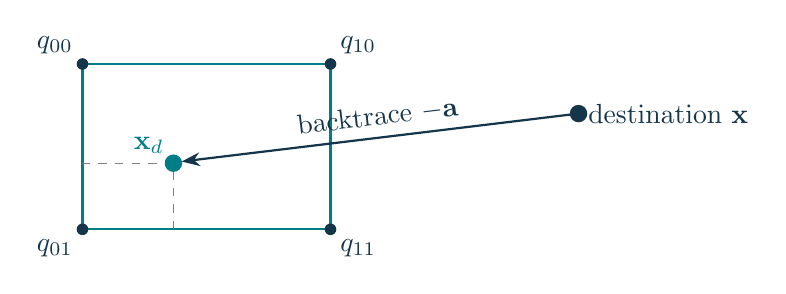
\begin{tikzpicture}[scale=1.05,>=Stealth]
\draw[teal,thick] (0,0) rectangle (3,2);
\fill[ink] (0,0) circle (2pt) node[below left] {$q_{01}$};
\fill[ink] (3,0) circle (2pt) node[below right] {$q_{11}$};
\fill[ink] (0,2) circle (2pt) node[above left] {$q_{00}$};
\fill[ink] (3,2) circle (2pt) node[above right] {$q_{10}$};
\draw[dashed,gray] (1.1,0)--(1.1,0.8)--(0,0.8);
\fill[teal] (1.1,0.8) circle (3pt) node[above left] {$\xvec_d$};
\draw[->,thick,ink] (6,1.4)--(1.2,0.82) node[midway,above,sloped] {backtrace $-\mathbf a$};
\fill[ink] (6,1.4) circle (3pt) node[right] {destination $\xvec$};
\end{tikzpicture}\par
{\footnotesize Schematic interpolation cell; the departure point can lie several cells away.}
\end{center}

\subsection*{Why this is useful, and what it costs}
The interpolation weights are nonnegative and sum to one. In exact arithmetic,
this sampling step with $0\leq r\leq1$ cannot increase the maximum absolute
value of any sampled component. This avoids the usual explicit-advection stability
restriction that a parcel move less than roughly one cell per step.

It does not make large steps accurate. A straight backtrace ignores trajectory
curvature, repeated interpolation blurs fine dye filaments and vortices, and the
method does not conserve the sum of dye values. No higher-order tracing,
MacCormack/BFECC correction, or conservative flux transport is present.
The stability argument applies to this sampling operation, not to the whole
solver with forces, finite precision, and approximate projection.
\src{\code{Shaders.metal}: \code{advect} and \code{bilerpFrag}.}

\page{User input and the meaning of Fade}
For a contact at grid position $\mathbf z_k$, the shader uses
\begin{equation}
 g_k(\xvec)=\exp\!\left(-\frac{\|\xvec-\mathbf z_k\|^2}{R}\right),\qquad
 \uvec\leftarrow\uvec+\sum_k\mathbf I_k g_k,\quad
 c\leftarrow c+\sum_k d\,g_k.\label{eq:splat}
\end{equation}
$\mathbf I_k=F\,\Delta\mathbf p_k/s_g$ is the supplied view-space displacement
multiplied by Force and converted to grid units; $d$ is Dye. The contact position
is likewise $\mathbf z_k=\mathbf p_k/s_g$. There is no division by elapsed event time, no integration
of force over seconds, and no normalization of the Gaussian's total integral.

Despite its name, \code{inkRadius} is the denominator $R$, not a radius or a
standard deviation. The $e^{-1}$ distance is $\sqrt R$, and the equivalent
Gaussian standard deviation is $\sqrt{R/2}$. At the default $R=150$, these are
about $12.25$ and $8.66$ grid cells. Increasing $R$ also increases total deposited
dye: on an infinite continuous plane, $\int g\,dA=\pi R$.

For mouse input the active renderer supplies $R=150/s_g$. For touch input it
uses $R=150(\min(\text{view width},\text{view height})/375)^2$, with the short
side clamped to at least one point. At the current $s_g=1$, the touch footprint
therefore scales with screen size. \code{SimulationTuning.radius} exists but is
not read by this active path.

Contacts occupy ten uniform slots per pass; extra contacts are split into
additional batches, each with a velocity pass and a dye pass. An unused slot is
marked by position $(0,0)$; \code{writeContacts} nudges a retained origin contact
to $(0.01,0.01)$ before grid scaling. Queued taps have zero impulse but still
deposit dye. Mac drag increments are measured between draws. iOS supplies
event-to-event displacements; the renderer reuses the latest touch contacts
until an input update replaces them. Input is consequently frame/event-rate
dependent rather than a calibrated force measurement.

\subsection*{Retention is applied to both transported fields}
The scalar $r$ in equation \eqref{eq:advect} multiplies \emph{both} self-advected
velocity and advected dye. Fade therefore damps motion as well as colour.
For an isolated value affected only by retention, in exact arithmetic,
\begin{equation}
 q_n=r^nq_0,\qquad
 \lambda_{\mathrm{step}}=-\ln r,\qquad
 n_{1/2}=\frac{\ln(1/2)}{\ln r}.
\end{equation}
The nominal default $r=0.998$ gives a half-life of about $346$ steps, or $5.77$
seconds if every second contains 60 advancing frames. This is an illustrative
decay calculation, not a measured dye lifetime: transport, sources, rounding,
and display saturation change what is visible. The shader casts $r$ to
\code{half}; $0.998$ becomes approximately $0.998046875$ even before repeated
output rounding.

The view requests 60 frames per second, but the solver does not compensate for
missed frames. At 30 advancing frames per second, decay measured in seconds
roughly slows by a factor of two. Multiplicative damping is proportional to the
local value; physical viscosity instead depends on spatial curvature.
\src{\code{Renderer}: \code{writeContacts}, \code{nextBuffer}, input methods;
platform \code{RenderViewController}s; \code{gaussSplat}, \code{applyForceVector},
\code{applyForceScalar}, and \code{advect}.}

\page{Vorticity confinement and wall treatment}
Vorticity measures local rotation. In the shader's coordinate convention,
\begin{equation}
 \omega=\partial_xv-\partial_yu,\qquad
 \omega_{ij}=\tfrac12\bigl(v_{i+1,j}-v_{i-1,j}
                         -u_{i,j+1}+u_{i,j-1}\bigr).
\end{equation}
This is a central difference with unit grid spacing. The visual interpretation
of its sign must respect the downward texture $y$ direction.

Semi-Lagrangian interpolation weakens small vortices. Confinement adds a force
constructed from variation in the \emph{magnitude} of vorticity, intended to
retain more rotational detail. Define
\begin{align}
 \boldsymbol\eta_{ij}
 &=\tfrac12\begin{pmatrix}
 |\omega_{i+1,j}|-|\omega_{i-1,j}|\\
 |\omega_{i,j+1}|-|\omega_{i,j-1}|
 \end{pmatrix},\\
 \mathbf f_{\mathrm{conf}}
 &=\frac{S\,\omega_{ij}}{\sqrt{\max(\epsilon,\|\boldsymbol\eta_{ij}\|^2)}}
 \begin{pmatrix}\eta_y\\-\eta_x\end{pmatrix},
 \qquad\epsilon=2.4414\times10^{-4},\label{eq:conf}\\
 \mathbf w&=B\bigl(\uvec^b+\mathbf f_{\mathrm{conf}}\bigr).
\end{align}
$S$ is Swirl (default $0.4$), and $B$ is the boundary overwrite below. In code,
the two gradient components are constructed in reversed order and the second
force component is negated. Equation \eqref{eq:conf} is that exact algebra,
equivalent to a regularized two-dimensional form of $\mathbf N\times\boldsymbol\omega$.
The denominator clamps the \emph{squared} norm before taking its square root;
it is not $\|\boldsymbol\eta\|+\epsilon$.

This force is artificial. It adds rotational motion but does not reconstruct
eddies lost below grid resolution or conserve kinetic energy. Uniform
$|\omega|$ gives zero force; a large Swirl setting is not a physical turbulence
parameter. The local shader time multiplier is explicitly $1.0$.

\subsection*{Two distinct boundary mechanisms}
First, simulation samplers specify nearest filtering but omit addressing and
coordinate modes. Metal's defaults are normalized coordinates and
\code{clamp\_to\_edge} (Apple MSL specification, section 2.10, table 2.7).
Samples beyond an edge thus reuse edge texels. Backtraces do not wrap around the
domain; the outer pressure neighbour is effectively the edge pressure itself.

Second, confinement and final gradient subtraction explicitly set \emph{both}
velocity components to zero wherever
\begin{equation}
 x\leq1\;\lor\;y\leq1\;\lor\;x\geq W-1\;\lor\;y\geq H-1.
\end{equation}
At texel centres on an ordinary grid this is the outermost row/column, a
no-slip-like border. The other passes do not enforce this overwrite, and dye is
not explicitly zeroed at walls. Edge clamping and this velocity mask are a
pragmatic boundary treatment, not a consistent ghost-cell discretization of all
wall conditions. The final overwrite can itself alter nearby divergence.
\src{\code{Shaders.metal}: \code{vorticity}, \code{vorticityConfinement},
\code{gradient}, and sampler declarations. External default:
\href{https://developer.apple.com/metal/Metal-Shading-Language-Specification.pdf}{Apple MSL specification}.}

\page{Pressure as a velocity correction}
Advection and forcing generally leave provisional velocity $\mathbf w$ with
nonzero divergence. The ideal projection subtracts a gradient,
\begin{equation}
 \uvec^{n+1}=\mathbf w-\nabla\phi,\qquad
 \nabla^2\phi=\nabla\cdot\mathbf w.\label{eq:projection}
\end{equation}
Taking the divergence of the first equation derives the second if the result is
to satisfy $\nabla\cdot\uvec^{n+1}=0$. In physical units one could set
$\phi=(\Delta t/\rho_0)p$. Here the code stores the scaled correction directly,
with unit step and cell conventions; it is not pressure in pascals.

\subsection*{Step 1: form the right-hand side}
For $\mathbf w=(w^x,w^y)$, the \code{divergence} shader computes
\begin{equation}
 b_{ij}=D_h\mathbf w
 =\tfrac12\left(w^x_{i+1,j}-w^x_{i-1,j}
                +w^y_{i,j+1}-w^y_{i,j-1}\right).
 \label{eq:divergence}
\end{equation}
$b$ is stored once for the pressure loop. Positive divergence means local
outflow exceeds inflow under this discrete measure.

\subsection*{Step 2: approximately solve a five-point Poisson equation}
The pressure iteration targets
\begin{equation}
 L_5\phi=\phi_{i-1,j}+\phi_{i+1,j}+\phi_{i,j-1}+\phi_{i,j+1}
 -4\phi_{ij}=b_{ij}.
\end{equation}
Rearranging for the centre value gives the Jacobi update used by \code{jacobi}:
\begin{equation}
 \boxed{\displaystyle
 \phi_{ij}^{(k+1)}=\frac{\phi_{i-1,j}^{(k)}+\phi_{i+1,j}^{(k)}
 +\phi_{i,j-1}^{(k)}+\phi_{i,j+1}^{(k)}-b_{ij}}{4}}
 \qquad k=0,\ldots,39.\label{eq:jacobi}
\end{equation}
This explains the shader constants \code{alpha = -1} and \code{beta = 4}.
All cells read iteration $k$ from one texture and write iteration $k+1$ to
another. This is Jacobi, not Gauss--Seidel, because no newly computed neighbour
is read in the same iteration.

The renderer retains the previous pressure texture between frames: it is a warm
start, not a fresh zero guess on every frame. The loop is literally
\code{0..<40}; \code{SimulationTuning.pressureIterations} is not consulted.
There is no residual-based stopping criterion.

\subsection*{Step 3: subtract the central-difference gradient}
\begin{equation}
 G_h\phi=\tfrac12
 \begin{pmatrix}\phi_{i+1,j}-\phi_{i-1,j}\\
                 \phi_{i,j+1}-\phi_{i,j-1}\end{pmatrix},\qquad
 \uvec^{n+1}=B\left(\mathbf w-G_h\phi^{(40)}\right).
 \label{eq:gradient}
\end{equation}
The pressure display reads this last iterate. It is a useful diagnostic of the
correction pattern, but does not establish a converged physical pressure field.
\src{\code{Shaders.metal}: \code{divergence}, \code{jacobi}, \code{gradient};
\code{Renderer.draw(in:)}: pressure loop.}

\page{Why the result is only approximately incompressible}
There are two independent reasons the pressure operation does not guarantee a
zero-divergence grid velocity. First, 40 Jacobi steps only approximate a solve.
Second, even a perfectly converged solve uses a Laplacian that does not equal
the composition of the actual divergence and gradient operators.

\subsection*{A stencil mismatch visible directly in the shaders}
Away from boundaries, composing the two central differences gives
\begin{equation}
 D_hG_h\phi=
 \frac{\phi_{i+2,j}+\phi_{i-2,j}+\phi_{i,j+2}+\phi_{i,j-2}-4\phi_{ij}}{4}.
 \label{eq:composed}
\end{equation}
This reaches neighbours \emph{two} cells away, whereas $L_5$ in the Jacobi solve
reaches neighbours one cell away. Both approximate a continuum Laplacian on
smooth fields, but they are different discrete operators.

Define the algebraic residual after the pressure solve as
$\mathcal R=b-L_5\phi$. Before the final boundary overwrite, equations
\eqref{eq:divergence} and \eqref{eq:gradient} imply
\begin{equation}
 D_h(\mathbf w-G_h\phi)
 =\underbrace{\mathcal R}_{\text{incomplete solve}}
  +\underbrace{(L_5-D_hG_h)\phi}_{\text{operator mismatch}}.
 \label{eq:residual}
\end{equation}
Thus more pressure iterations alone do not remove all measured divergence.
For an interior checkerboard $\phi_{ij}=(-1)^{i+j}$, for example,
$G_h\phi=0$ while $L_5\phi=-8\phi$. This illustrates the grid-scale decoupling
possible with collocated central differences; it is a mathematical example,
not a claim that a particular app frame contains that pattern.

\subsection*{Boundaries, convergence, and conservation}
Clamped pressure sampling resembles a zero-normal-gradient extension. Such
Neumann-like systems leave the constant pressure offset undetermined. The code
does not pin a pressure value, subtract its mean, or explicitly enforce the
right-hand-side compatibility condition. Velocity depends on gradients, but the
pressure visualization can still depend on its offset.

Jacobi is local and simple to parallelize, but long-wavelength error relaxes
slowly. A fixed count gives predictable work, not grid-independent accuracy;
larger grids do not receive more iterations. Half-precision arithmetic further
limits small corrections. The final zero-velocity border adds another source of
discrete divergence near the wall.

\note{\textbf{What is sacrificed for visualization.} The scheme does not promise
exact dye-mass conservation, exact incompressibility, momentum conservation, or
energy conservation. Advection interpolation, retention, user injection,
confinement, wall overwrites, and half-precision storage all affect these
quantities. There is no quantitative error tolerance or adaptive refinement.}

These limitations do not prevent compelling swirling dye. They do mean that
visual plausibility must not be interpreted as a validated prediction of a
physical flow. A consistent discrete projection, convergence monitoring, and a
specified physical timestep would be separate numerical design changes.
\src{Algebra derived from the \code{divergence}, \code{jacobi}, and
\code{gradient} stencils; no empirical error measurement is asserted.}

\page{Making each step practical on the GPU}
\subsection*{Textures as arrays; drawing as computation}
Each slab owns two \code{rg16Float} textures, called \code{ping} and
\code{pong}. The renderer draws a full-screen quad (two indexed triangles) into
\code{pong}; a fragment invocation computes each destination cell from
\code{ping}. Swapping the references makes the output the next input.
This avoids reading and writing the same texture in one pass and makes Jacobi's
iteration dependency explicit. The active simulation uses render passes, not
the project's separate \code{ComputeShader} helper.

With $B_c$ contact batches and an available drawable, an ordinary advancing
frame uses
\begin{equation}
 \underbrace{2}_{\text{advection}}
 +\underbrace{2B_c}_{\text{input}}
 +\underbrace{2}_{\text{curl + confinement}}
 +\underbrace{1}_{\text{divergence}}
 +\underbrace{40}_{\text{pressure}}
 +\underbrace{1}_{\text{gradient}}
 +\underbrace{1}_{\text{display}}=47+2B_c
\end{equation}
render passes. With one contact batch this is 49. Most work is local texture
sampling; the 40 pressure passes dominate the pass count. The work scales
roughly as $O(WH(40+B_c+1))$, with up to ten splats evaluated per input pass.
This is a cost model, not a measured frame-rate claim.

Five double-buffered slabs at two 16-bit channels per texel require nominally
$5\times2\times4WH=40WH$ bytes of field storage, excluding alignment, uniforms,
drawables, and transient resize textures. Scalars still occupy two channels.
Half storage reduces memory traffic relative to 32-bit channels but has limited
range and precision. Some shaders calculate in \code{float}; splats, much of
Jacobi, and final outputs use \code{half}. Rounding occurs between passes.

\subsection*{Initial values and scheduling}
\code{Slab.init} allocates textures but performs no explicit clear or upload.
\code{RenderShader} sets \code{loadAction = .dontCare}; its black
\code{clearColor} is therefore not an initialization pass. From source alone,
one should not claim a solver-defined zero initial condition. A reproducible
numerical experiment would explicitly initialize all fields before sampling
them. The warm-start description applies once a pressure result has been stored.

Three uniform buffers and a semaphore permit up to three frames in flight,
while command buffers use the same command queue. This is scheduling overlap;
it does not mean three independent fluid states are simulated.

\subsection*{Resizing preserves an image-space state}
The resize pass nearest-samples each old field at normalized coordinates. For
velocity only, it applies componentwise scale factors,
\begin{equation}
 u_{\rm new}(\boldsymbol\xi)=\frac{W_{\rm new}}{W_{\rm old}}
 u_{\rm old}(\boldsymbol\xi),\qquad
 v_{\rm new}(\boldsymbol\xi)=\frac{H_{\rm new}}{H_{\rm old}}
 v_{\rm old}(\boldsymbol\xi).
\end{equation}
This preserves displacement as a fraction of the canvas per step. Other fields
are copied without amplitude scaling. No conservative remap or immediate
reprojection occurs; copied divergence/vorticity need not be derivatives of the
resized velocity. They are recomputed on the next advancing frame. Input is
cleared and new grid offsets are installed.
\src{\code{Slab.swift}, \code{RenderShader.swift}, \code{Renderer.swift},
\code{MetalDevice.swift}; \code{Shaders.metal}: \code{resampleField}.}

\page{What the controls and colours mean}
\subsection*{The displayed field is not a calibrated plot}
Density and Pressure use the first texture channel $q$ and map it to
\begin{equation}
 (R,G,B,A)=\left(0,\;0.06|q|,\;0.19|q|,\;1\right).
\end{equation}
The absolute value discards pressure sign. Brightness is not normalized to the
range of the field. On the \code{bgra8Unorm} output target, channels clamp to
$[0,1]$ and are quantized, so blue saturates at $|q|\simeq5.26$ and green at
$|q|\simeq16.67$ in ideal arithmetic.

Velocity \emph{and Vorticity} use \code{visualizeVector}, whose expression is
\begin{equation}
 \mathbf C=\tfrac12\mathbf 1+\tfrac12\mathbf q.
\end{equation}
Velocity therefore places $u$ in red and $v$ in green, centred on mid-grey for
zero components; it is not a vector-arrow or speed-magnitude plot. Vorticity is
actually scalar, stored as $(\omega,0)$, so its red channel varies with signed
$\omega$ and its green channel stays at $0.5$. Values outside $[-1,1]$ clip in
these displayed channels. The same sample conversion also handles the unused
blue/alpha components.

The stored vorticity was computed \emph{before} confinement and projection in
the frame. It is not a recomputed curl of the final displayed velocity.
Divergence has no selectable display field, and selecting a field changes only
the presentation, not the evolving simulation.

\subsection*{Slider position versus numerical value}
For normalized slider position $z\in[0,1]$, Force, Dye, and Swirl each map to
$2z$. Fade maps to retention by the following piecewise rule:
\begin{equation}
 r(z)=\begin{cases}
 0.9995-0.0015(z/0.17), & z<0.17,\\
 0.998, & z=0.17,\\
 0.998-0.0075((z-0.17)/0.83), & z>0.17.
 \end{cases}
\end{equation}
The central equality is explicitly special-cased in Swift. The UI range is
$0.9905\leq r\leq0.9995$: even minimum Fade retains less than one, and maximum
Fade does not immediately erase a field.

\begin{tabularx}{\linewidth}{@{}lclY@{}}
\toprule
Control & Default UI & Default value & Effect \\
\midrule
Force & 50\% & $F=1$ & Multiplies contact displacement. \\
Dye & 40\% & $d=0.8$ & Adds dye per contact per advancing frame. \\
Swirl & 20\% & $S=0.4$ & Scales confinement of existing vorticity. \\
Fade & 17\% & $r=0.998$ & Retains velocity and dye during advection. \\
\bottomrule
\end{tabularx}

Radius and pressure-iteration properties exist in \code{SimulationTuning}, but
the live pipeline chooses radius through its input paths and hard-codes 40
iterations. There is no runtime resolution control. Changing the source grid
scale alone would also require care with force, splat width, timestep, and
projection accuracy if consistent physical behaviour were the goal.
\src{\code{SimulationState.swift}: \code{SimulationTuning}; \code{Renderer}:
\code{render}, \code{drawSlab}; \code{visualizeScalar}, \code{visualizeVector}.}

\page{Source map and reproducibility}
All paths below are relative to the repository root. Function names are given
instead of line numbers so that small unrelated edits do not invalidate the map.
The description was checked against simulation sources at commit
\code{9477dabc41a24780371c07e8decb7a9ba3d337a0}.

{\small
\begin{tabularx}{\linewidth}{@{}>{\raggedright\arraybackslash}p{0.43\linewidth}Y@{}}
\toprule
File & What to inspect \\
\midrule
\path{Sources/Shared/Renderer.swift} & \code{draw(in:)} for order and 40 iterations;
\code{writeContacts}/\code{nextBuffer} for input; resize callback for grid size
and remapping; \code{render} for field-to-shader selection. \\
\path{Sources/Shared/Shaders.metal} & \code{advect}/\code{bilerpFrag}; force shaders;
\code{vorticity}/\code{vorticityConfinement}; \code{divergence}/\code{jacobi}/\code{gradient};
visualizers and \code{resampleField}. These define the discrete equations. \\
\path{Sources/Shared/Slab.swift} & Texture formats, paired allocation, and swapping. \\
\path{Sources/Shared/RenderShader.swift} & Full-quad render passes and load/store actions. \\
\path{Sources/Shared/MetalDevice.swift} & Shared device, queue, and pipeline creation. \\
\path{Sources/Shared/SimulationState.swift} & Slider mappings, defaults, and advance/pause state. \\
\path{Sources/macOS/}\newline\code{RenderViewController.swift} & Mouse position conversion and forwarding. \\
\path{Sources/iOS/}\newline\code{RenderViewController.swift} & \code{submitTouches} displacement construction;
tap and hold handling. \\
\bottomrule
\end{tabularx}\par
}

\subsection*{Evidence and limits}
The equations here are transcriptions or algebraic consequences of the source,
with ordinary fluid mechanics used to explain their purpose. The document does
not report a new GPU benchmark, conservation test, or convergence study.
Existing \path{Tests/Integration/test_phase05_metal.swift} exercises shader
responses to force, dye, retention, and swirl; \path{test_phase03_metal.swift}
in the same directory exercises resize remapping. Those checks are not a proof
of Navier--Stokes accuracy or discrete incompressibility.

\subsection*{Optional primary references}
\begin{itemize}
\item Apple, \emph{Metal Shading Language Specification}, 4 June 2026,
section 2.10, table 2.7: sampler defaults used on page 6.
\href{https://developer.apple.com/metal/Metal-Shading-Language-Specification.pdf}{Official specification PDF}.
\item Mark J. Harris, \emph{GPU Gems}, chapter 38, ``Fast Fluid Dynamics
Simulation on the GPU'' (2004).
\href{https://developer.nvidia.com/gpugems/gpugems/part-vi-beyond-triangles/chapter-38-fast-fluid-dynamics-simulation-gpu}{Current NVIDIA chapter page}.
This is background reading; its algorithm should not be substituted for this
repository's exact implementation.
\end{itemize}

\subsection*{Rebuild the document}
The editable source and generated PDF live together in \path{docs/}.
From the repository root, with a LaTeX distribution providing the packages named
in the preamble, run:
\begin{quote}\small\ttfamily
latexmk -pdf -interaction=nonstopmode -halt-on-error \textbackslash\\
\hspace*{1em}-outdir=docs docs/fluid-dynamics.tex
\end{quote}
\end{document}
